\subsection{Node analysis for $t\geq0$ - natural solution for $v_6(t)$}
Analysing now the circuit in $t>0$ in order to determine the evolution of the voltage on node 6, $V_6$, with time, $v_6(t)$, one can start by determining its natural solution. To do that, we start by assuming the general form of this solution which can be written as:

\begin{equation}
    v_{6n}(t) = v_{6n} (t\to\infty) + (v_{6n}(t = 0) - v_{6n}(t\to\infty))e^{-\frac{t}{\tau}}
\label{generalfor}
\end{equation}

in which $\tau$ represents the time constant for this RC circuit, i.e., $\tau = R_{eq}C$, as calculated on the previous section.\\

Starting by $v_6 (t=0)$, the initial condition for the solution which we are seeking is $V_x$, the voltage obtained in the last section for the voltage source by which one replaced the capacitor. So on, using the last section results, as $V_x = V_6 - V_8$ and $V_8 = 0$, one can infer that $V_x = V_6$, and so one can conclude that $v_6(t=0) = V_x$. \\

Only $v_(t\to\infty)$ remains unknows. To find it, one can run again the nodal analysis system of equations with $V_s = 0$, as we are searching only for the natural solution by now. So, one can write the equivalent matricial equation for $t\to\infty$ as:

\begin{equation}
    \begin{bmatrix}
     1 &  0      &  0 &    -1  &     0      &  0  &  0    &  0\\
     -G_1 & G_1+G_2+G_3 & -G_2  & 0   &  -G_3       &  0  &  0    &  0\\
     0   & -G_2-K_b    & G_2  & 0   &   K_b       &  0  &  0    &  0\\
     0   & 0        & 0   & 1 & 0       &  0  & 0   & 0\\
     0   & -G_3+K_b      &  0 &  -G_4  &   G_3+G_4-K_b & 0 &  -G_7    & G_7\\
     0   & 0       & 0  &  0    & 0     & 1  & 0     & -1\\
     0   & K_b        & 0  & 0   &  -G_5-K_b         & G_5   & 0 & 0\\
     0   & 0        & 0  &  -K_dG_6    &  1         & 0   & K_dG_6     & -1
    \end{bmatrix} 
    \begin{bmatrix}
        V_1\\
        V_2\\
        V_3\\
        V_4\\
        V_5\\
        V_6\\
        V_7\\
        V_8
    \end{bmatrix}
    = 
    \begin{bmatrix}
        0\\
        0\\
        0\\
        0\\
        0\\
        0\\
        0\\
        0
    \end{bmatrix}
\label{eqnodos}
\end{equation}

which results in the following solution:

\begin{equation}
    \begin{bmatrix}
        V_1\\
        V_2\\
        V_3\\
        V_4\\
        V_5\\
        V_6\\
        V_7\\
        V_8
    \end{bmatrix}
    = 
    \begin{bmatrix}
        0\\
        0\\
        0\\
        0\\
        0\\
        0\\
        0\\
        0
    \end{bmatrix} V
\label{zeros}
\end{equation}

Knowing $v_{6n}(t = 0)$ and $v_{6n}(t\to\infty)$ one can now use equation \eqref{generalfor} to find the expression for the natural solution of the voltage on node 6:

\begin{equation}
    v_{6n}(t) \approx 8.4036e^{-\frac{t}{0.0030516}}
\end{equation}

Plotting the function obtained on the interval $t \in [0,20]ms$, one can get the graph shown in Fig. \ref{fig:natural}

\begin{figure}[H]
    \centering
    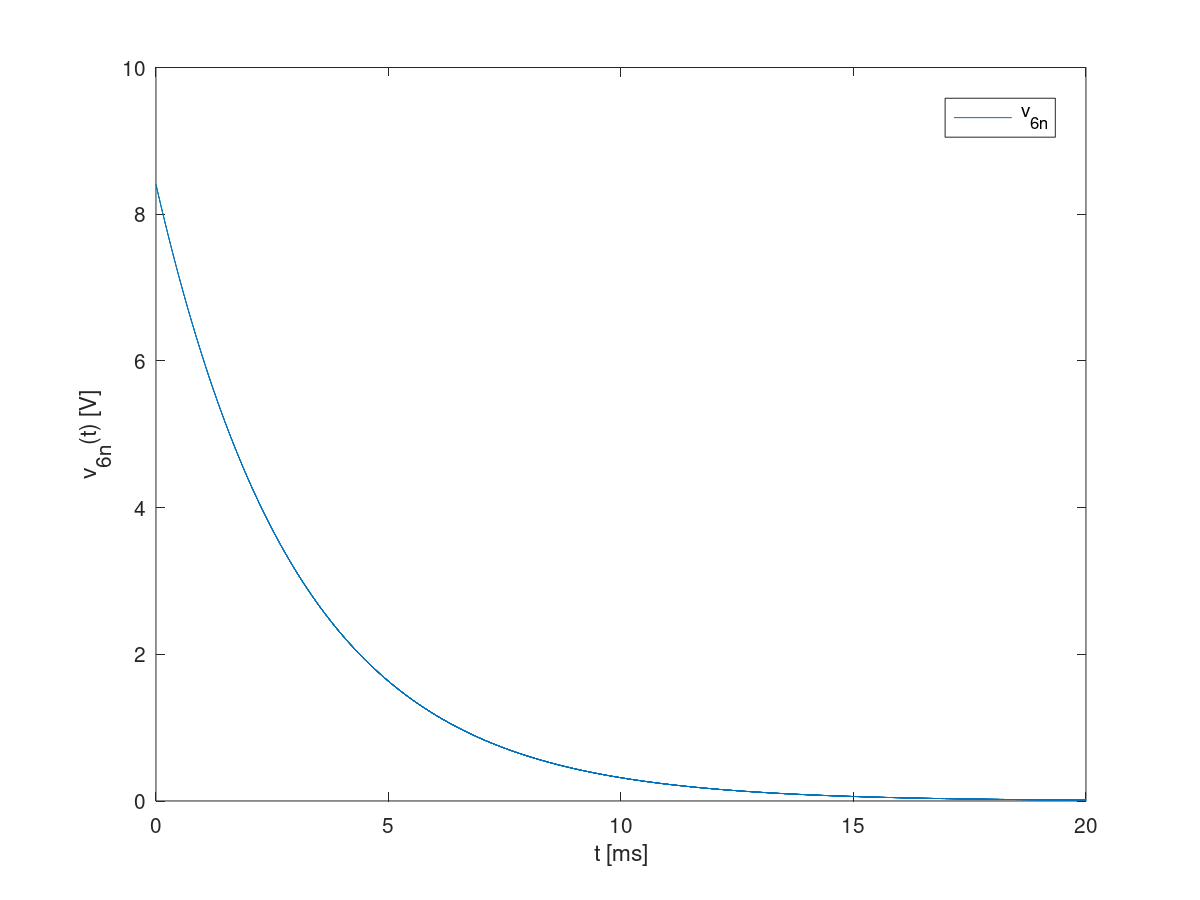
\includegraphics[width = 0.85\linewidth]{../mat/v6n.png}
        \caption{\textit{Plot of the natural solution for the voltage on node 6 in the interval $t\in[0,20]ms$ as shown on the plot}}
    \label{fig:natural}
\end{figure}